%!TEX root = da2020-04.tex

\Chapter{4}{\tLOCAL{}~Model: Unique~Identifiers}

\noindent
In the previous chapter, we studied deterministic distributed algorithms in port-numbered networks. In this chapter we will study a stronger model: \emph{networks with unique identifiers}\mydash see Figure~\ref{fig:unique-ids}. Following the standard terminology of the field, we will use the term ``$\LOCAL$ model'' to refer to networks with unique identifiers.

\begin{figure}
    \centering
    \includegraphics[page=\PUniqueIds]{figs.pdf}
    \caption{A network with unique identifiers.}\label{fig:unique-ids}
\end{figure}


\section{Definitions}\label{sec:unique-id}

Throughout this chapter, fix a constant $c > 1$. An assignment of \emph{unique identifiers} for a port-numbered network $N = (V,P,p)$ is an injection
\[
    \Id \colon V \to \{1,2, \dotsc, |V|^c\}.
\]
That is, each node $v \in V$ is labeled with a unique integer, and the labels are assumed to be relatively small.

Formally, unique identifiers can be interpreted as a graph problem $\Pi'$, where each solution $\Id \in \Pi'(N)$ is an assignment of unique identifiers for network $N$. If a distributed algorithm $A$ solves a problem $\Pi$ on a family $\calF$ given $\Pi'$, we say that \emph{$A$ solves $\Pi$ on $\calF$ given unique identifiers}, or equivalently, \emph{$A$ solves $\Pi$ on $\calF$ in the $\LOCAL$ model}.

For the sake of convenience, when we discuss networks with unique identifiers, we will identify a node with its unique identifier, i.e., $v = \Id(v)$ for all $v \in V$.


\section{Gathering Everything}\label{sec:gather}

In the $\LOCAL$ model, if the underlying graph $G = (V,E)$ is connected, all nodes can learn everything about $G$ in time $O(\diam(G))$. In this section, we will present a gathering algorithm that accomplishes this.

In the gathering algorithm, each node $v \in V$ will construct sets $V(v,r)$ and $E(v,r)$, where $r = 1, 2, \dotsc$. For all $v \in V$ and $r \ge 1$, these sets will satisfy
\begin{align}
    V(v,r) &= \ball_G(v,r), \label{eq:gather1} \\
    E(v,r) &= \bigl\{ \{s,t\} : s \in \ball_G(v,r),\, t\in \ball_G(v,r{-}1) \bigr\}. \label{eq:gather2}
\intertext{Now define the graph}
    G(v,r) &= (V(v,r), E(v,r)).  \label{eq:gather3}
\end{align}
See Figure~\ref{fig:gather} for an illustration.

\begin{figure}
    \centering
    \includegraphics[page=\PGather]{figs.pdf}
    \caption{Subgraph $G(v,r)$ defined in \eqref{eq:gather3}, for $v = 14$ and $r = 2$.}\label{fig:gather}
\end{figure}

The following properties are straightforward corollaries of \eqref{eq:gather1}--\eqref{eq:gather3}.
\begin{enumerate}
    \item Graph $G(v,r)$ is a subgraph of $G(v,r+1)$, which is a subgraph of~$G$.
    \item If $G$ is a connected graph, and $r \ge \diam(G) + 1$, we have $G(v,r) = G$.
    \item If $G_v$ is the connected component of $G$ that contains $v$, and $r \ge \diam(G_v) + 1$, we have $G(v,r) = G_v$.
    \item For a sufficiently large $r$, we have $G(v,r) = G(v,r+1)$.
    \item If $G(v,r) = G(v,r+1)$, we will also have $G(v,r+1) = G(v,r+2)$.
    \item Graph $G(v,r)$ for $r > 1$ can be constructed recursively as follows:
    \begin{align}
        V(v,r) &= \bigcup_{u \in V(v,1)} V(u,r-1), \label{eq:Vvr} \\
        E(v,r) &= \bigcup_{u \in V(v,1)} E(u,r-1). \label{eq:Evr}
    \end{align}
\end{enumerate} 

The gathering algorithm maintains the following invariant: after round $r \ge 1$, each node $v \in V$ has constructed graph $G(v,r)$. The execution of the algorithm proceeds as follows:
\begin{enumerate}
    \item In round $1$, each node $u \in V$ sends its identity $u$ to each of its ports. Hence after round $1$, each node $v \in V$ knows its own identity and the identities of its neighbors. Put otherwise, $v$ knows precisely $G(v,1)$.
    \item In round $r > 1$, each node $u \in V$ sends $G(u,r-1)$ to each of its ports. Hence after round $r$, each node $v \in V$ knows $G(u,r-1)$ for all $u \in V(v,1)$. Now $v$ can reconstruct $G(v,r)$ using \eqref{eq:Vvr} and \eqref{eq:Evr}.
    \item A node $v \in V$ can stop once it detects that the graph $G(v,r)$ no longer changes.
\end{enumerate}

It is easy to extend the gathering algorithm so that we can discover not only the underlying graph $G = (V,E)$ but also the original port-numbered network $N = (V,P,p)$.


\section{Solving Everything}

Let $\calF$ be a family of connected graphs, and let $\Pi$ be a distributed graph problem. Assume that there is a deterministic \emph{centralized} (non-distributed) algorithm $A'$ that solves $\Pi$ on $\calF$. For example, $A'$ can be a simple brute-force algorithm\mydash we are not interested in the running time of algorithm~$A'$.

Now there is a simple distributed algorithm $A$ that solves $\Pi$ on $\calF$ in the $\LOCAL$ model. Let $N = (V,P,p)$ be a port-numbered network with the underlying graph $G \in \calF$. Algorithm $A$ proceeds as follows.
\begin{enumerate}
    \item All nodes discover $N$ using the gathering algorithm from Section~\ref{sec:gather}.
    \item All nodes use the centralized algorithm $A'$ to find a solution $f \in \Pi(N)$. From the perspective of algorithm $A$, this is merely a state transition; it is a local step that requires no communication at all, and hence takes $0$ communication rounds.
    \item Finally, each node $v \in V$ switches to state $f(v)$ and stops.
\end{enumerate}
Clearly, the running time of the algorithm is $O(\diam(G))$.

It is essential that all nodes have the same canonical representation of network $N$ (for example, $V$, $P$, and $p$ are represented as lists that are ordered lexicographically by node identifiers and port numbers), and that all nodes use the same deterministic algorithm $A'$ to solve $\Pi$. This way we are guaranteed that all nodes have locally computed the \emph{same} solution $f$, and hence the outputs $f(v)$ are globally consistent.


\section{Focus on Computational Complexity}

So far we have learned the key difference between $\PN$ and $\LOCAL$ models: while there are plenty of graph problems that cannot be solved at all in the $\PN$ model, we know that all computable graph problems can be easily solved in the $\LOCAL$ model.

Hence our focus shifts from computability to computational complexity. While it is trivial to determine if a problem can be solved in the $\LOCAL$ model, we would like to know which problems can be solved quickly. In particular, we would like to learn which problems can be solved in time that is much smaller than $\diam(G)$. It turns out that graph coloring is an example of such a problem.

In the rest of this chapter, we will design an efficient distributed algorithm that finds a graph coloring in the $\LOCAL$ model. The algorithm will find a proper vertex coloring with $\Delta+1$ colors in $O(\Delta + \log^* n)$ communication rounds, for any graph with $n = |V|$ nodes and maximum degree $\Delta$. We will start with a simple greedy algorithm that we will later use as a subroutine.


\section{Greedy Color Reduction} \label{sec:bdgreedy}

Let $x \in \NN$. We present a greedy color reduction algorithm that reduces the number of colors from $x$ to
\[
    y = \max \{ x-1, \Delta+1 \},
\]
where $\Delta$ is the maximum degree of the graph. That is, given a proper vertex coloring with $x$ colors, the algorithm outputs a proper vertex coloring with $y$ colors. The running time of the algorithm is one communication round.

\subsection{Algorithm}

The algorithm proceeds as follows; here $f$ is the $x$-coloring that we are given as input and $g$ is the $y$-coloring that we produce as output. See Figure~\ref{fig:greedy} for an illustration.
\begin{enumerate}
    \item In the first communication round, each node $v \in V$ sends its color $f(v)$ to each of its neighbors.
    \item Now each node $v \in V$ knows the set
    \[
        C(v) = \{ i : \text{there is a neighbor $u$ of $v$ with $f(u) = i$} \}.
    \]
    We say that a node is \emph{active} if $f(v) > \max C(v)$; otherwise it is \emph{passive}. That is, the colors of the active nodes are local maxima. Let
    \[
        \bar{C}(v) = \{1,2,\dotsc\} \setminus C(v)
    \]
    be the set of \emph{free colors} in the neighborhood of $v$.
    \item A node $v \in V$ outputs
    \[
        g(v) = \begin{cases}
            f(v) & \text{if $v$ is passive}, \\
            \min \bar{C}(v) & \text{if $v$ is active}.
        \end{cases}
    \]
\end{enumerate}
Informally, a node whose color is a local maximum re-colors itself with the first available free color.

\begin{figure}
    \centering
    \includegraphics[page=\PGreedy]{figs.pdf}
    \caption{Greedy color reduction. The active nodes have been highlighted. Note that in the original coloring $f$, the largest color was $99$, while in the new coloring, the largest color is strictly smaller than $99$\mydash we have successfully reduced the number of colors in the graph.}\label{fig:greedy}
\end{figure}

\subsection{Analysis}

\begin{lemma}
    The greedy color reduction algorithm reduces the number of colors from $x$ to
    \[
        y = \max \{ x-1, \Delta+1 \},
    \]
    where $\Delta$ is the maximum degree of the graph.
\end{lemma}
\begin{proof}
    Let us first prove that $g(v) \in \{1,2,\dotsc,y\}$ for all $v \in V$. As $f$ is a proper coloring, we cannot have $f(v) = \max C(v)$. Hence there are only two possibilities.
    \begin{enumerate}
        \item $f(v) < \max C(v)$. Now $v$ is passive, and it is adjacent to a node $u$ such that $f(v) < f(u)$. We have
        \[
            g(v) = f(v) \le f(u) - 1 \le x - 1 \le y.
        \]
        \item $f(v) > \max C(v)$. Now $v$ is active, and we have
        \[
            g(v) = \min \bar{C}(v).
        \]
        There is at least one value $i \in \{1,2,\dotsc,|C(v)|+1\}$ with $i \notin C(v)$; hence
        \[
            \min \bar{C}(v) \le |C(v)| + 1 \le \deg_G(v) + 1 \le \Delta + 1 \le y.
        \]
    \end{enumerate}
    
    Next we will show that $g$ is a proper vertex coloring of $G$. Let $\{u,v\} \in E$. If both $u$ and $v$ are passive, we have
    \[
        g(u) = f(u) \ne f(v) = g(v).
    \]
    Otherwise, w.l.o.g., assume that $u$ is active. Then we must have $f(u) > f(v)$. It follows that $f(u) \in C(v)$ and $f(v) \le \max C(v)$; therefore $v$ is passive. Now
    $g(u) \notin C(u)$ while
    $g(v) = f(v) \in C(u)$; we have $g(u) \ne g(v)$.
\end{proof}

The key observation is that the set of active nodes forms an independent set. Therefore all active nodes can pick their new colors simultaneously in parallel, without any risk of choosing colors that might conflict with each other.

\subsection{Remarks}

The greedy color reduction algorithm does not need to know the number of colors $x$ or the maximum degree $\Delta$; we only used them in the analysis. We can take any graph, blindly apply greedy color reduction, and we are guaranteed to reduce the number of colors by one\mydash provided that the number of colors was larger than $\Delta + 1$. In particular, we can apply the greedy color reduction repeatedly until we get stuck, at which point we have a \Dpocol{} of~$G$\mydash we will formalize and generalize this idea in Exercise~\ref{ex:greedy-iterate}.

\section[{Efficient \texorpdfstring{$(\Delta+1)$}{(Δ+1)}-coloring}]{\boldmath Efficient $(\Delta+1)$-coloring}

In the remaining sections we will describe two coloring algorithms that, together with the greedy algorithm from the previous section, can be used to $(\Delta+1)$-color graphs of maximum degree $\Delta$.

On a high level, the $(\Delta+1)$-coloring algorithm is composed of the following subroutines:
\begin{enumerate}
  \item Algorithm from Section~\ref{sec:delta2-coloring}: Using unique identifiers as input, compute an $O(\Delta^2)$-coloring $x$ in $O(\log^* n)$ rounds.
  \item Algorithm from Section~\ref{sec:additive-group-col}: Given $x$ as input, compute an $O(\Delta)$-coloring $y$ in $O(\Delta)$ rounds.
  \item Algorithm from Section~\ref{sec:bdgreedy}: Given $y$ as input, compute a $(\Delta+1)$-coloring $z$ in $O(\Delta)$ rounds.
\end{enumerate}
We have already seen the greedy algorithm that we will use in the final step; we will proceed in the reverse order and present next the algorithm that turns an $O(\Delta^2)$-coloring into an $O(\Delta)$-coloring. In what follows, we will assume that the nodes are given the values of $\Delta$ and $n$ as input; these assumptions will simplify the algorithms significantly.

\section{Additive-Group Coloring} \label{sec:additive-group-col}

Consider two clocks with $q$ steps, for any prime $q$; see Figure~\ref{fig:clocks}. The first clock moves its hand $a$ steps in each time unit, and the second clock moves its hand $b \neq a$ steps in each time unit. Starting from the same position, when are the two hands in the same position again?

\begin{figure}
    \centering
    \includegraphics[scale=0.25,page=\PClocks]{figs.pdf}
    \caption{Two clocks for $q=7$. The blue hand moves 2 steps per time unit, and the orange hand 3 steps. Hands moving at different speeds meet again after $q$ moves, but not before.}\label{fig:clocks}
\end{figure}

It is a fundamental property of \emph{finite fields} that they are in the same position again after exactly $q$ steps. We recap definitions and facts about finite fields in Section~\ref{app:finite-fields}.

Building on this observation, we construct an algorithm where each node behaves like a clock with one hand, turning its hand with some constant speed. We will use the input coloring to ensure that \emph{clocks with the same starting position turn their hands at different speeds}. Then we will simply wait until a clock is in a position not shared by any of the neighbors, and this position becomes the final color of the node. If we do not have too many neighbors, each node will eventually find such a position, leading to a proper coloring.

\subsection{Algorithm}\label{sec:additive-group-col-alg}

Let $q$ be a prime number with $q > 2\Delta$. We assume that we are given a coloring with $q^2$ colors, and we will show how to construct a coloring with $q$ colors in $O(q)$ rounds. Put otherwise, we can turn a coloring with $O(\Delta^2)$ colors into a coloring with $O(\Delta)$ colors in $O(\Delta)$ rounds, as long as we choose our prime number $q$ in a suitable manner.

If we have an input coloring with $q^2$ colors, we can represent the color of node $v$ as a pair $f(v) = \langle f_1(v), f_2(v) \rangle$ where $f_1(v)$ and $f_2(v)$ are integers between $0$ and $q-1$.

Using the clock analogue, $v$ can be seen as a clock with the hand at position $f_2(v)$, turning at speed $f_1(v)$. In the algorithm we will stop clocks by setting $f_1(v) = 0$ whenever this is possible in a conflict-free manner. When all clocks have stopped, all nodes have colors of the form $\langle 0, f_2(v) \rangle$ where $f_2(v)$ is between $0$ and $q-1$, and hence we have got a proper coloring with $q$ colors.

We say that two colors $\langle a_1, a_2 \rangle$ and $\langle b_1, b_2 \rangle$ are in \emph{conflict} if $a_2 = b_2$. The algorithm repeatedly performs the following steps:
\begin{itemize}[noitemsep]
  \item Each node sends its current colors to each neighbor.
  \item For each node $v$, if $f(v)$ is in conflict with any neighbor, set
  \begin{align*}
    f(v) &\gets \bigl\langle f_1(v),\, (f_1(v) + f_2(v)) \bmod q \bigr\rangle.
  \intertext{Otherwise, set}
    f(v) &\gets \bigl\langle 0,\, f_2(v) \bigr\rangle.
  \end{align*}
\end{itemize}
In essence, we stop non-conflicting clocks and keep moving all other clocks at a constant rate. We say that a node $v$ is \emph{stopped} when $f_1(v) = 0$; otherwise it is \emph{running}; note a stopped node will not change its color any more.

We show that after $O(q)$ iterations of this loop, all nodes will be stopped, and they form a proper coloring\mydash assuming we started with a proper coloring.

\subsection{Correctness}

First, we show that in each iteration a proper coloring remains proper. In what follows, we use $f$ to denote the coloring before one iteration and $g$ to denote the coloring after the iteration. Consider a fixed node $v$ and an arbitrary neighbor $u$. We show by a case analysis that $f(v) \neq f(u)$ implies $g(v) \neq g(u)$.
\begin{enumerate}[label=(\arabic*)]
  \item Assume that $v$ is stopped after this round; then $g(v) = \langle 0, f_2(v) \rangle$.
  \begin{enumerate}
    \item If $f_1(u) = 0$, then $u$ has stopped and $g(u) = f(u)$. By assumption $f(v) \neq f(u)$ and therefore $g(v) \neq g(u)$.
    \item If $f_1(u) \neq 0$ and $f(u)$ is not in conflict with its neighbors, then $g(u) = \langle 0, f_2(u) \rangle$. As there are no conflicts with $v$, we must have $f_2(v) \neq f_2(u)$, and therefore $g(v) \neq g(u)$.
    \item Otherwise $f_1(u) \neq 0$ and $f(u)$ is in conflict with a neighboring color. Then $g_1(u) = f_1(u) \neq 0 = g_1(v)$, and therefore $g(v) \neq g(u)$.
  \end{enumerate}
  \item Otherwise we have $g(v) = \langle f_1(v), (f_1(v) + f_2(v)) \bmod q \rangle$, where $f_1(v) \ne 0$.
  \begin{enumerate}
    \item If $u$ has stopped, then $g_1(u) = 0$, and therefore $g(v) \neq g(u)$.
    \item Otherwise $u$ is running. Then \[g(u) = \langle f_1(u), (f_1(u)+f_2(u)) \bmod q \rangle.\] If $f_1(v) \ne f_1(u)$, we will have $g_1(v) \ne g_1(u)$ and therefore $g(v) \ne g(u)$. Otherwise $f_1(v) = f_1(u)$ but then by assumption we must have $f_2(v) \ne f_2(u)$, which implies $g_2(v) \ne g_2(u)$ and therefore $g(v) \ne g(u)$.
  \end{enumerate}
\end{enumerate}

\subsection{Running Time}

Next we analyze the running time. Assume that we start with a proper coloring $f$. We want to show that after a sufficient number of iterations of the additive-group algorithm, each node must have had an iteration in which its color did not conflict with color of its neighbors, and hence got an opportunity to stop.

Let $f^0$ denote the initial coloring before the first iteration and let $f^i$ denote the coloring after iteration $i = 1, 2, \dotsc$. The following lemma shows that two running nodes do not conflict too often during the execution.

\begin{lemma} \label{lem:agc-running-conflict}
  Consider $t$ consecutive iterations of the additive-group coloring algorithm, for $t \leq q$. Let $u$ and $v$ be adjacent nodes such that both of them are still running before iteration $t$. Then there is at most one iteration $i = 0, 1, \dotsc, t-1$ with a conflict $f_2^i(u) = f_2^i(v)$.
\end{lemma}

\begin{proof}
  Assume that for some $i$ we have $f^i(u) = \langle a, b \rangle$ and $f^i(v) = \langle a', b \rangle$ with $a \ne a'$. In the subsequent iterations $j=i+1,i+2,\dots$, we have
  \[
    f^j_2(u) - f^j_2(v) \equiv (a-a')(j-i) \mod q.
  \]
  Assume that for some $j$ we have another conflict $f^j_2(u) = f^j_2(v)$, implying that $(a-a')(j-i) \equiv 0 \mod q$. If a prime divides a product $xy$ of two integers $x$ and $y$, then it also divides $x$ or $y$ (Euclid's Lemma). But $a-a'$ cannot be a multiple of $q$, since $a \ne a'$ and $0 \le a, a' < q$, and $j-i$ cannot be a multiple of $q$, either, since $0 \le i < j < q$.
\end{proof}

We also need to show that a node is not in conflict with a stopped node too often.

\begin{lemma} \label{lem:agc-finished-conflict}
  Consider $t$ consecutive iterations of the additive-group coloring algorithm, for $t \leq q$. Let $u$ and $v$ be adjacent nodes such that $u$ is still running before iteration $t$ but $v$ was stopped before iteration $1$. Then there is at most one iteration $i = 0, 1, \dotsc, t-1$ with a conflict $f_2^i(u) = f_2^i(v)$.
\end{lemma}

\begin{proof}
  The same argument as in the proof of Lemma~\ref{lem:agc-running-conflict} works, this time with $a' = 0$.
\end{proof}

It remains to show that, based on Lemmas~\ref{lem:agc-running-conflict} and \ref{lem:agc-finished-conflict}, the algorithm finishes fast.

Consider a sequence of consecutive $q > 2\Delta$ iterations of the additive-group coloring algorithm starting with any initial coloring $f$. Consider an arbitrary node $u$ that does not stop during any of these rounds. Let $v$ be a neighbor of $u$. No matter if and when $v$ stops, the color of $v$ will conflict with color of $u$ at most twice during the $q$ rounds:
\begin{itemize}
    \item Consider the rounds (if any) in which $v$ is running. There are at most $q$ such rounds. By Lemma~\ref{lem:agc-running-conflict}, $u$ conflicts with $v$ at most once during these rounds.
    \item Consider the remaining rounds (if any) in which $v$ is stopped. There are at most $q$ such rounds. By Lemma~\ref{lem:agc-finished-conflict}, $u$ conflicts with $v$ at most once during these rounds.
\end{itemize}
So for each neighbor $v$ of $u$, there are at most $2$ rounds among $q$ rounds such that the color of $v$ conflicts with the color of $u$. As there are at most $\Delta$ neighbors, there are at most $2\Delta$ rounds among $q$ rounds such that the color of some neighbor of $u$ conflicts with the current color of $u$. But $q > 2\Delta$, so there has to be at least one round after which none of the neighbors are in conflict with $u$---and hence there will be an opportunity for $u$ to stop.

\section[Fast \texorpdfstring{$O(\Delta^2)$}{O(Δ²)}-coloring]{\boldmath Fast $O(\Delta^2)$-coloring} \label{sec:delta2-coloring}

The additive-group coloring algorithm assumes that we start with an $O(\Delta^2)$-coloring of the network. In this section we present an algorithm that computes an $O(\Delta^2)$-coloring in $O(\log^* n)$ communication rounds.

The algorithm proceeds in two phases. In the first phase, the coloring given by the unique identifiers is iteratively reduced to an $O(\Delta^2 \log^2 \Delta)$-coloring. In the second phase, a final color reduction step yields an $O(\Delta^2)$ coloring.

Both phases are based on the same combinatorial construction, called a cover-free set family. We begin by describing the construction for the first phase.

\subsection{Cover-Free Set Families}

The coloring algorithm is based on the existence of non-covering families of sets. Intuitively, these are families of sets such that any two sets do not have a large overlap: then no small collection of sets contains all elements in another set. Therefore, if each node is assigned such a set, it can find an element that is not in the sets of its neighbors, and pick that element as its new color.

\begin{figure}
  \centering
  \includegraphics[scale=0.4,page=\PCoverFreeSet]{figs.pdf}
  \caption{A 2-cover-free set family $J$ of 5 subsets of a base set $X$ on 7 elements. No two sets cover a third distinct set.}\label{fig:cover-free-sets}
\end{figure}

A family $J$ of $n$ subsets of $\{1, \dots, m \}$ is \emph{$k$-cover-free} if for every $S \in J$ and every collection of $k$ sets $S_1, \dots, S_k \in J$ distinct from $S$ we have that
\[
  S \nsubseteq \bigcup_{i=1}^{k} S_i.
\]
See Figure~\ref{fig:cover-free-sets} for an example.

\subsection{Constructing Cover-Free Set Families}

Cover-free set families can be constructed using \emph{polynomials over finite fields}. The example of finite fields we are interested in is $\GF(q)$ for a prime $q$, which is simply modular arithmetic of integers modulo $q$. We consider polynomials over such a field. A brief recap is given in Section~\ref{app:finite-fields}.

A basic result about polynomials states that two distinct polynomials evaluate to the same value at a bounded number of points

\begin{lemma} \label{lem:poly-roots}
  Let $f,g$ be two distinct polynomials of degree $d$ over a finite field $\GF(q)$, for some prime $q$. Then $f(x) = g(x)$ holds for at most $d$ elements $x \in \GF(q)$.
\end{lemma}
\begin{proof}
See Section~\ref{app:finite-fields}.
\end{proof}

Now fix a prime $q$. Our base set will be $X = \GF(q) \times \GF(q)$. Thus we have that $|X| = m = q^2$.

For a positive natural number $d$, consider $\Poly(d,q)$, the set of polynomials of degree $d$ over $\GF(q)$. For each polynomial $g \in \Poly(d,q)$, fix the set \[S_g = \bigl\{ (a, g(a)) \bigm| a \in \GF(q) \bigr\}\] that is associated with this polynomial. Note that each $S_g$ contains exactly $q$ elements: one for each element of $\GF(q)$. Then we can define the family \[J = J_{d,q} = \bigl\{ S_g \bigm| g \in \Poly(d,q) \bigr\}.\]

Consider any two distinct polynomials $f$ and $g$ in $\Poly(d,q)$: by Lemma~\ref{lem:poly-roots} there are at most $d$ elements $a$ such that $f(a) = g(a)$. Therefore $|S_f \cap S_g| \leq d$, and $J$ is a $\lfloor q/d \rfloor$-cover-free set family.

Any polynomial is uniquely defined by its coefficients. Therefore the set $J_{d,q}$ has size $q^{d+1}$, as it consists of a set of pairs for each polynomial of degree $d$.

By choosing parameters $q$ and $d$ we can construct a $\Delta$-cover free family that can be used to color efficiently.

\begin{lemma} \label{lem:delta-cover-free}
  For all integers $x$, $\Delta$ such that $x > \Delta \geq 2$, there exists a $\Delta$-cover-free family $J$ of $x$ subsets from a base set of $m \leq 4(\Delta+1)^2 \log^2 x$ elements.
\end{lemma}

\begin{proof}
  We begin by choosing a prime $q$ such that
  \[
    \bigl\lfloor (\Delta+1)\log x \bigr\rfloor \leq q \leq 2 \cdot \bigl\lfloor (\Delta+1)\log x \bigr\rfloor.
  \]
  By the Bertrand--Chebyshev theorem such a prime must always exist. Set $d = \lfloor \log x \rfloor$. By the previous observation, the family $J_{d,q}$, for the above parameter settings, is a $\lfloor q / d \rfloor$-cover-free family, where 
  \[
    \lfloor q / d \rfloor \geq \biggl\lfloor \frac{\lfloor (\Delta+1)\log x \rfloor}{\lfloor \log x \rfloor} \biggr\rfloor \geq \biggl\lfloor \frac{(\Delta+1)\log x - 1}{\log x} \biggr\rfloor \geq \Delta.
  \]
  There are at least 
  \[
  q^{d+1} \geq (\Delta \log x)^{\log x } > x
  \]
  sets in $J_{d,q}$, so we can choose $x$ of them. The base set has \[q^2 \leq 4(\Delta+1)^2 \log^2 x\] elements.
\end{proof}

\subsection{Efficient Color Reduction} \label{ssec:efficient-cr}

Using $\Delta$-cover-free sets we can construct an algorithm that reduces the number of colors from $x$ to $y \leq 4(\Delta+1)^2 \log^2 x$ in one communication round, as long as $x > \Delta$.

Let $f$ denote the input $x$-coloring and $g$ the output $y$-coloring. Assume that $J$ is a $\Delta$-cover-free family of $x$ sets on a base set of $y$ elements, as in Lemma~\ref{lem:delta-cover-free}, that is ordered as $S_1, S_2, \dots, S_x$. The algorithm functions as follows.
\begin{enumerate}
  \item Each node $v \in V$ sends its current color $f(v)$ to each of its neighbors.
  \item Each node receives the colors $f(u)$ of its neighbors $u \in N(v)$. Then it constructs the set $S_{f(v)}$, and the sets $S_{f(u)}$ for all $u \in N(v)$. Since $f(v) \neq f(u)$ for all $u\in N(v)$, and $J$ is a $\Delta$-cover-free family, we have that
  \[
    S_{f(v)} \nsubseteq \bigcup_{u \in N(v)} S_{f(u)}.
  \]
  In particular, there exists at least one $c \in S_{f(v)} \setminus \cup_{u \in N(v)} S_{f(u)}$. Node $v$ sets $g(v) = c$ for the smallest such $c$.
\end{enumerate}

Now assume that $f$ is a proper coloring, that is, $f(v) \neq f(u)$ for all neighbors $v$ and $u$. This implies that for each node $v$, each of its neighbors $u$ selects a set that is different from $S_{f(v)}$; overall, the neighbors will select at most $\Delta$ distinct sets. Since $J$ is a $\Delta$-cover-free family, each node $v$ can find an element $c \in S_{f(v)}$ that is not in the sets of its neighbors. Therefore setting $g(v) = c$ forms a proper coloring. Finally, since the sets $S \in J$ are subsets of $\{1,\dots,y\}$, for $y \leq 4(\Delta+1)^2 (\log x)^2$, we have that $g$ is a $y$-coloring.

\subsection{Iterated Color Reduction}

By a repeated application of the color reduction algorithm it is possible to reduce the number of colors down to $O(\Delta^2 \log^2 \Delta)$. Assuming we start with an input $x$-coloring, this will take $O(\log^* x)$ rounds.

We will now show that $O(\log^* x)$ iterations of the color reduction algorithm will reduce the number of colors from $x$ to $O(\Delta^2 \log^2 \Delta)$. We assume that in the beginning, both $x$ and $\Delta$ are known. Therefore after each iteration, all nodes know the total number of colors.

Assume that $x > 4(\Delta+1)^2 \log^2 \Delta$. Repeated iterations of the color reduction algorithm reduce the number of colors as follows:
\begin{align*}
  x_0 \mapsto x_1 &\leq 4(\Delta+1)^2 \log^2 x, \\
  x_1 \mapsto x_2 &\leq 4(\Delta+1)^2 \log^2 (4(\Delta+1)^2 \log^2 x) \\
  & {} = 4(\Delta+1)^2 \bigl(\log 4 + 2\log (\Delta+1) + 2\log \log x\bigr)^2.
\intertext{If $\log \log x \geq \log 4 + 2\log (\Delta+1)$, we have that}
  x_2 & \leq 4(\Delta+1)^2(3\log \log x)^2 \\
  &= \bigl(6 (\Delta+1) \log \log x\bigr)^2.
\intertext{In the next step, we reduce colors as follows:}
  x_2 \mapsto  x_3 &\leq 4(\Delta+1)^2 \log^2 \bigl(36(\Delta+1)^2 (\log \log x)^2\bigr) \\
  & = 4(\Delta+1)^2 \bigl(\log 36 + 2\log (\Delta+1) + 2\log \log \log x\bigr)^2.
\intertext{If $\log \log \log x \geq \log 36 + 2\log (\Delta+1) \}$, we have that}
  x_3 &\leq 4(\Delta+1)^2(3\log \log \log x)^2 \\
  &= \bigl(6(\Delta+1) \log \log \log x\bigr)^2.
\end{align*}
Now we can see the pattern: as long as 
\[
\log^{(i)} x \geq \log 36 + 2\log (\Delta+1) \},
\] 
where $\log^{(i)} x$ is the $i$ times iterated logarithm of $x$, we reduce colors from $(6(\Delta+1)\log^{(i-1)} x)^2$ to $(6(\Delta+1)\log^{(i)} x)^2$ in the $i$th step.

Once $\log^{(i)} x \geq \log 36 + 2\log (\Delta+1) \}$ no longer holds, we have a coloring with at most 
\[
c_{\Delta} = 4(\Delta+1)^2 \bigl(3(\log 36 + 2\log (\Delta+1))\bigr)^2
\] 
colors. We can numerically verify that for all $\Delta \geq 2$, we have that
\[
  4(\Delta+1)^2 \bigl(3(\log 36 + 2\log (\Delta+1))\bigr)^2 \leq (11(\Delta+1))^3.
\]
We will use this observation in the next step.

It remains to calculate how many color reduction steps are required. By definition, after $T = \log^* x$ iterations we have that $\log^{(T)} x \leq 1$. Thus, after at most $\log^* x$ iterations of the color reduction algorithm we have a coloring with at most $c_{\Delta}$ colors.

\subsection{Final Color Reduction Step} \label{ssec:final-step}

In the last step, we will reduce the coloring to an $O(\Delta^2)$-coloring. We will use another construction of $\Delta$-cover-free families based on polynomials.

\begin{lemma} \label{lem:delta3-to-delta2}
  For all $\Delta$, there exists a $\Delta$-cover-free family $J$ of $x$ subsets from a base set of $m \le (22(\Delta+1))^2$ elements for $x \leq (11(\Delta+1))^3$.
\end{lemma}

This immediately gives us the following color reduction algorithm.

\begin{corollary}
  There is a distributed algorithm that, given a $(11(\Delta+1))^3$-coloring as an input, in one round computes a $(22(\Delta+1))^2$-coloring.
\end{corollary}

\begin{proof}[Proof of Lemma~\ref{lem:delta3-to-delta2}]
  Our base set will be $X$ with $|X| = m = q^2$, for a prime $q$. Again it is useful to see $X = \GF(q) \times \GF(q)$ as pairs of elements from the finite field over $q$ elements.
  
  Now consider polynomials $\Poly(2,q)$ of degree 2 over $\GF(q)$. For each such polynomial $g \in \Poly(2,q)$, let 
  \[
    S_g = \bigl\{ (a, g(a)) \bigm| a \in \GF(q) \bigr\}
  \]
  be the pairs defined by the valuations of the polynomial $g$ at each element of $\GF(q)$. We have that $|S_g| = q$ for all $g$.
  
  Now we can construct the family \[J = J_{2,q} = \bigl\{ S_g \bigm| g \in \Poly(2,q) \bigr\}\] as the collection of point sets defined by all polynomials of degree 2. We have that $|J| = q^3$ since a polynomial is uniquely determined by its coefficients.
  
  By Lemma~\ref{lem:poly-roots}, we have that $|S_f \cap S_g| \leq 2$ for any distinct polynomials $f,g \in P(2,q)$. Therefore covering any set $S_g$ requires at least $\lceil q/2 \rceil$ other sets (distinct from $S_g$) from $J$.
  
  We are now ready to prove that $J$ is a $\Delta$-cover-free family for suitable parameter settings. Since each set $S_g$ contains $q$ elements, and the intersection between the sets of distinct polynomials is at most $2$, we want to find $q$ such that $2\Delta \leq q - 1$ and $q^3$ is large enough. Using the Bertrand--Chebyshev theorem we know that there exists a prime $q$ such that
  \[
    11(\Delta + 1) \leq q \leq 22(\Delta + 1).
  \]
  Any value $q$ from this range is large enough. The base set $X$ has size 
  \[
  m = q^2 \leq (22(\Delta + 1))^2.
  \]
  The family $J$ has size
  \[
    |J| \geq (11(\Delta + 1))^3.
  \]
  Finally, since we choose $q \geq 2\Delta + 1$, we have that no collection of $\Delta$ sets $\mathcal{S} = \{ S_1, S_2, \dots, S_{\Delta} \} \subseteq J$ can cover a set $S \notin \mathcal{S}$.
\end{proof}

\section{Putting Things Together}

It remains to show how to use the three algorithms we have seen so far together.

\begin{theorem}
  Assume that we know parameters $\Delta$ and $n$, and some polynomial bound $n^c$ on the size of the unique identifiers. Graphs on $n$ vertices with maximum degree $\Delta$ can be $(\Delta+1)$-colored in $O(\Delta + \log^* n)$ rounds in the $\LOCAL$ model.
\end{theorem}

\begin{proof}
  We begin with the unique identifiers, and treat them as an initial coloring with $n^c$ colors. 
  \begin{enumerate}
    \item In the first phase we run the efficient color reduction algorithm from Section~\ref{ssec:efficient-cr} for $T_1 = \log^* (n^c) = O(\log^* n)$ rounds to produce a coloring $y_1$ with at most $(11(\Delta+1))^3$ colors.
    \item In the second phase, after $T_1$ rounds have passed, each vertex can apply the final color reduction step from Section~\ref{ssec:final-step} to compute a coloring $y_2$. This reduces colors from $(11(\Delta+1))^3$ to $(22(\Delta+1))^2$.
    \item After $T_1 + 1$ rounds, we have computed an $O(\Delta^2)$-coloring $y_2$. Now each vertex runs the additive-group coloring algorithm from Section~\ref{sec:additive-group-col}, applying it with $y_2$ as input. For a parameter $q \leq 2\sqrt{(22(\Delta+1))^2} = 44\Delta+44$, this algorithm runs for $T_2 = q$ steps and computes a $q$-coloring $y_3$.
    \item In the last phase, after $T_1 + 1 + T_2$ rounds, we apply the greedy color reduction algorithm from Section~\ref{sec:bdgreedy} iteratively $T_3 = 43\Delta+43$ times. Each iteration requires one round and reduces the maximum color by one.
  \end{enumerate}
  After a total of
  \begin{align*}
      T_1 + 1 + T_2 + T_3 &\leq \log^* (n^c) + 87\Delta + 88 \\
      &= O(\Delta + \log^* n)
  \end{align*}
  rounds, we have computed a $(\Delta+1)$-coloring.
\end{proof}

\section{Quiz}

Consider the algorithm from Section~\ref{sec:additive-group-col-alg} in the following setting:
\begin{itemize}[noitemsep]
    \item The network is a complete graph with $n = 4$ nodes; hence the maximum degree is $\Delta = 3$, and we can choose $q = 7 > 2\Delta$.
    \item We are given a coloring with $q^2 = 49$ colors; we can represent the possible input colors as pairs $(0,0),\allowbreak (0,1),\allowbreak \dotsc,\allowbreak (6,6)$.
\end{itemize}
Give an example of an input coloring such that we need to do exactly $6$ iterations of the algorithm until all nodes have reached their final colors, i.e., colors of the form $(0,x)$.

Please give the answer by listing the four original color pairs of the nodes in any order; for example, if we asked for a coloring in which you need exactly 3 iterations, this would be a correct answer: $(2, 3)$, $(3, 2)$, $(3, 6)$, $(4, 6)$.

\section{Exercises}

\begin{ex}[applications]
    Let $\Delta$ be a known constant, and let $\calF$ be the family of graphs of maximum degree at most $\Delta$. Design fast distributed algorithms that solve the following problems on $\calF$ in the $\LOCAL$ model.
    \begin{subex}
        \item Maximal independent set.
        \item Maximal matching.
        \item Edge coloring with $O(\Delta)$ colors.
    \end{subex}
    You can assume that all nodes get the value of $n$ as input; also the parameter $c$ in the identifier space is a known constant, so all nodes know the range of unique identifiers.
\end{ex}

\begin{ex}[vertex cover]
    Let $\calF$ consist of cycle graphs. Design a fast distributed algorithm that finds a \Apx{1.1} of a minimum vertex cover on $\calF$ in the $\LOCAL$ model.
    
    \hint{Solve small problem instances by brute force and focus on the case of long cycles. In a long cycle, use a graph coloring algorithm to find a $3$-coloring, and then use the $3$-coloring to construct a maximal independent set. Observe that a maximal independent set partitions the cycle into short fragments (with 2--3 nodes in each fragment).

    Apply the same approach recursively: interpret each fragment as a ``supernode'' and partition the cycle that is formed by the supernodes into short fragments, etc. Eventually, you have partitioned the original cycle into \emph{long} fragments, with dozens of nodes in each fragment.
    
    Find an optimal vertex cover within each fragment. Make sure that the solution is feasible near the boundaries, and prove that you are able to achieve the required approximation ratio.}
\end{ex}

\begin{ex}[iterated greedy]\label{ex:greedy-iterate}
    Design a color reduction algorithm $A$ with the following properties:
    given any graph $G = (V,E)$ and any proper vertex coloring~$f$,
    algorithm $A$ outputs a proper vertex coloring~$g$ such that
    for each node $v \in V$ we have $g(v) \le \deg_G(v) + 1$.
    
    Let $\Delta$ be the maximum degree of $G$, let $n = |V|$ be the number of nodes in $G$, and let $x$ be the number of colors in coloring $f$. The running time of $A$ should be at most
    \[
        \min \{ n, x \} + O(1).
    \]
    Note that the algorithm does not know $n$, $x$, or $\Delta$. Also note that we may have either $x \le n$ or $x \ge n$.
    
    \hint{Adapt the basic idea of the greedy color reduction algorithm\mydash find local maxima and choose appropriate colors for them\mydash but pay attention to the stopping conditions and low-degree nodes. One possible strategy is this: a node becomes active if its current color is a local maximum among those neighbors that have not yet stopped; once a node becomes active, it selects an appropriate color and stops.}
\end{ex}

\begin{ex}[distance-$2$ coloring]\label{ex:distance2col}
    Let $G = (V,E)$ be a graph. A \emph{distance-$2$ coloring with $k$ colors} is a function $f \colon V \to \{1,2,\dotsc,k\}$ with the following property:
    \[
        \dist_G(u,v) \le 2 \text{ implies } f(u) \ne f(v) \text{ for all nodes } u \ne v.
    \]

    Let $\Delta$ be a known constant, and let $\calF$ be the family of graphs of maximum degree at most $\Delta$. Design a fast distributed algorithm that finds a distance-$2$ coloring with $O(\Delta^2)$ colors for any graph $G \in \calF$ in the $\LOCAL$ model.

    You can assume that all nodes get the value of $n$ as input; also the parameter $c$ in the identifier space is a known constant, so all nodes know the range of unique identifiers.

    \hint{Given a graph $G \in \calF$, construct a virtual graph $G^2 = (V, E')$ as follows: $\{u,v\} \in E'$ if $u \ne v$ and $\dist_G(u,v) \le 2$. Prove that the maximum degree of $G^2$ is $O(\Delta^2)$. Simulate a fast graph coloring algorithm on $G^2$.}
\end{ex}

\begin{exs}[numeral systems]\label{ex:dpbit-base}
    The fast color reduction algorithm from Section~\longref{1.4}{sec:algo-p3cbit} is based on the idea of identifying a digit that differs in the \emph{binary} encodings of the colors. Generalize the idea: design an analogous algorithm that finds a digit that differs in the base-$k$ encodings of the colors, for an arbitrary $k$, and analyze the running time of the algorithm (cf.\ Exercise~\longref{1.6}{ex:logstar-tight}). Is the special case of $k = 2$ the best possible choice?
\end{exs}

\begin{exs}[from bits to sets]\label{ex:dpset}
    The fast color reduction algorithm from Section~\longref{1.4}{sec:algo-p3cbit} can reduce the number of colors from $2^x$ to $2x$ in one round in any directed pseudoforest, for any positive integer $x$. For example, we can reduce the number of colors as follows:
    \[
        2^{128} \to 256 \to 16 \to 8 \to 6.
    \]
    One of the problems is that an iterated application of the algorithm slows down and eventually ``gets stuck'' at $x = 3$, i.e., at six colors.
    
    In this exercise we will design a faster color reduction algorithm that reduces the number of colors from
    \[
        h(x) = \binom{2x}{x}
    \]
    to $2x$ in one round, for any positive integer $x$. For example, we can reduce the number of colors as follows:
    \[
        184756 \to 20 \to 6 \to 4.
    \]
    Here
    \begin{align*}
        184756 &= h(10), \\
        2 \cdot 10 = 20 &= h(3), \\
        2 \cdot 3 = 6 &= h(2).
    \end{align*}
    In particular, the algorithm does not get stuck at six colors; we can use the same algorithm to reduce the number of colors to four. Moreover, at least in this case the algorithm seems to be much more efficient\mydash it can reduce the number of colors from $184756$ to $6$ in two rounds, while the prior algorithm requires at three rounds to achieve the same reduction.
    
    The basic structure of the new algorithm follows the fast color reduction algorithm\mydash in particular, we use one communication round to compute the values $s(v)$ for all nodes $v \in V$. However, the technique for choosing the new color is different: as the name suggests, we will not interpret colors as bit strings but as \emph{sets}.
    
    To this end, let $H(x)$ consist of all subsets
    \[
        X \subseteq \{1,2,\dotsc,2x\}
    \]
    with $|X| = x$. There are precisely $h(x)$ such subsets, and hence we can find a bijection
    \[
        L\colon \{1,2,\dotsc,h(x)\} \to H(x).
    \]
    
    We have $f(v) \ne s(v)$. Hence $L(f(v)) \ne L(s(v))$. As both $L(f(v))$ and $L(s(v))$ are subsets of size $x$, it follows that
    \[
        L(f(v)) \setminus L(s(v)) \ne \emptyset.
    \]
    We choose the new color $g(v)$ of a node $v \in V$ as follows:
    \[
        g(v) = \min \bigl( L(f(v)) \setminus L(s(v)) \bigr).
    \]

    Prove that this algorithm works correctly. In particular, show that $g\colon V \to \{1,2,\dotsc,2x\}$ is a proper graph coloring of the directed pseudoforest~$G$.
    
    Analyze the running time of the new algorithm and compare it with the old algorithm. Is the new algorithm always faster? Can you prove a general result analogous to the claim of Exercise~\longref{1.6}{ex:logstar-tight}?
\end{exs}


\begin{exs}[dominating set approximation]\label{ex:greedy-domset}
    Let $\Delta$ be a known constant, and let $\calF$ be the family of graphs of maximum degree at most $\Delta$. Design an algorithm that finds an \Apx{O(\log \Delta)} of a minimum dominating set on $\calF$ in the $\LOCAL$ model.
    
    \hint{First, design (or look up) a greedy \emph{centralized} algorithm achieves an approximation ratio of $O(\log \Delta)$ on $\calF$. The following idea will work: repeatedly pick a node that \emph{dominates} as many new nodes as possible\mydash here a node $v \in V$ is said to dominate all nodes in $\ball_G(v,1)$. For more details, see a textbook on approximation algorithms, e.g., Vazirani~\cite{vazirani01approximation}.
    
    Second, show that you can \emph{simulate} the centralized greedy algorithm in a distributed setting. Use the algorithm of Exercise~\ref{ex:distance2col} to construct a distance-$2$ coloring. Prove that the following strategy is a faithful simulation of the centralized greedy algorithm: 
    \begin{itemize}[label=--,noitemsep]
        \item For each possible value $i = \Delta+1, \Delta, \dotsc, 2, 1$:
        \begin{itemize}[label=--,nolistsep,topsep=1ex]
            \item For each color $j = 1, 2, \dotsc, O(\Delta^2)$:
            \begin{itemize}[label=--,nolistsep,topsep=1ex]
                \item Pick all nodes $v \in V$ that are of color $j$ and that dominate $i$ new nodes.
            \end{itemize}
        \end{itemize}
    \end{itemize}
    The key observation is that if $u,v \in V$ are two distinct nodes of the same color, then the set of nodes dominated by $u$ and the set of nodes dominated by $v$ are disjoint. Hence it does not matter whether the greedy algorithm picks $u$ before $v$ or $v$ before $u$, provided that both of them are equally good from the perspective of the number of new nodes that they dominate. Indeed, we can equally well pick both $u$ and $v$ simultaneously in parallel.}
\end{exs}


\section{Bibliographic Notes}

The model of computing is from Linial's~\cite{linial92locality} seminal paper, and the name $\LOCAL$ is from Peleg's~\cite{peleg00distributed} book. The additive-group coloring algorithm is due to Barenboim et al.\ \cite{barenboim18iterative}. The effective color reduction algorithm is from Linial~\cite{linial92locality}, and the construction of cover-free families from Barenboim and Elkin~\cite{barenboim13distributed}.
The algorithm of Exercise~\ref{ex:greedy-domset} is from Friedman and Kogan~\cite{friedman11deterministic}. The Bertrand--Chebyshev theorem was first proven by Chebyshev~\cite{chebyshev1852primes}. The proof of Lemma~\ref{lem:poly-roots} follows the proofs of Abraham~\cite{abraham2020polynomials}.

